\documentclass[journal,12pt,twocolumn]{IEEEtran}
\usepackage{setspace}
\usepackage{gensymb}
\usepackage{caption}
%\usepackage{multirow}
%\usepackage{multicolumn}
%\usepackage{subcaption}
%\doublespacing
\singlespacing
\usepackage{csvsimple}
\usepackage{amsmath}
\usepackage{multicol}
%\usepackage{enumerate}
\usepackage{amssymb}
%\usepackage{graphicx}
\usepackage{newfloat}
%\usepackage{syntax}
\usepackage{listings}
\usepackage{color}
\usepackage{tikz}
\usetikzlibrary{shapes,arrows}
%\usepackage{wasysym}
\usepackage{amsthm}
\usepackage{mathrsfs}
\usepackage{txfonts}
\usepackage{stfloats}
\usepackage{cite}
\usepackage{cases}
\usepackage{mathtools}
\usepackage{caption}
\usepackage{enumerate}	
\usepackage{enumitem}
\usepackage{amsmath}
%\usepackage{xtab}
\usepackage{longtable}
\usepackage{multirow}
%\usepackage{algorithm}
%\usepackage{algpseudocode}
\usepackage{enumitem}
\usepackage{mathtools}
\usepackage{hyperref}
%\usepackage[framemethod=tikz]{mdframed}
\usepackage{listings}
    %\usepackage[latin1]{inputenc}                                 %%
    \usepackage{color}                                            %%
    \usepackage{array}                                            %%
    \usepackage{longtable}                                        %%
    \usepackage{calc}                                             %%
    \usepackage{multirow}                                         %%
    \usepackage{hhline}                                           %%
    \usepackage{ifthen}                                           %%
  %optionally (for landscape tables embedded in another document): %%
    \usepackage{lscape}     


\usepackage{url}
\def\UrlBreaks{\do\/\do-}


%\usepackage{stmaryrd}


%\usepackage{wasysym}
%\newcounter{MYtempeqncnt}
% \renewcommand\vec{\mathbf}
\DeclareMathOperator*{\Res}{Res}
%\renewcommand{\baselinestretch}{2}
\renewcommand\thesection{\arabic{section}}
\renewcommand\thesubsection{\thesection.\arabic{subsection}}
\renewcommand\thesubsubsection{\thesubsection.\arabic{subsubsection}}

\renewcommand\thesectiondis{\arabic{section}}
\renewcommand\thesubsectiondis{\thesectiondis.\arabic{subsection}}
\renewcommand\thesubsubsectiondis{\thesubsectiondis.\arabic{subsubsection}}

% correct bad hyphenation here
\hyphenation{op-tical net-works semi-conduc-tor}

\lstset{
%language=C,
frame=single, 
breaklines=true,
columns=fullflexible
}
 

\begin{document}
%
\tikzstyle{block} = [rectangle, draw,
    text width=3em, text centered, minimum height=3em]
\tikzstyle{sum} = [draw, circle, node distance=3cm]
\tikzstyle{input} = [coordinate]
\tikzstyle{output} = [coordinate]
\tikzstyle{pinstyle} = [pin edge={to-,thin,black}]

\theoremstyle{definition}
\newtheorem{theorem}{Theorem}[section]
\newtheorem{problem}{Problem}
\newtheorem{proposition}{Proposition}[section]
\newtheorem{lemma}{Lemma}[section]
\newtheorem{corollary}[theorem]{Corollary}
\newtheorem{example}{Example}[section]
\newtheorem{definition}{Definition}[section]
%\newtheorem{algorithm}{Algorithm}[section]
%\newtheorem{cor}{Corollary}
\newcommand{\BEQA}{\begin{eqnarray}}
\newcommand{\EEQA}{\end{eqnarray}}
\newcommand{\define}{\stackrel{\triangle}{=}}

\bibliographystyle{IEEEtran}
%\bibliographystyle{ieeetr}

\providecommand{\nCr}[2]{\,^{#1}C_{#2}} % nCr
\providecommand{\nPr}[2]{\,^{#1}P_{#2}} % nPr
\providecommand{\mbf}{\mathbf}
\providecommand{\pr}[1]{\ensuremath{\Pr\left(#1\right)}}
\providecommand{\qfunc}[1]{\ensuremath{Q\left(#1\right)}}
\providecommand{\sbrak}[1]{\ensuremath{{}\left[#1\right]}}
\providecommand{\lsbrak}[1]{\ensuremath{{}\left[#1\right.}}
\providecommand{\rsbrak}[1]{\ensuremath{{}\left.#1\right]}}
\providecommand{\brak}[1]{\ensuremath{\left(#1\right)}}
\providecommand{\lbrak}[1]{\ensuremath{\left(#1\right.}}
\providecommand{\rbrak}[1]{\ensuremath{\left.#1\right)}}
\providecommand{\cbrak}[1]{\ensuremath{\left\{#1\right\}}}
\providecommand{\lcbrak}[1]{\ensuremath{\left\{#1\right.}}
\providecommand{\rcbrak}[1]{\ensuremath{\left.#1\right\}}}
\theoremstyle{remark}
\newtheorem{rem}{Remark}
\newcommand{\sgn}{\mathop{\mathrm{sgn}}}

\makeatletter
\@addtoreset{figure}{section}
\makeatother

\let\StandardTheFigure\thefigure
%\renewcommand{\thefigure}{\theproblem.\arabic{figure}}
\renewcommand{\thefigure}{\thesection}


%\numberwithin{figure}{subsection}

%\numberwithin{equation}{subsection}
%\numberwithin{equation}{section}
%\numberwithin{equation}{problem}
%\numberwithin{problem}{subsection}
\numberwithin{problem}{section}
%%\numberwithin{definition}{subsection}
%\makeatletter
%\@addtoreset{figure}{problem}
%\makeatother
\makeatletter
\@addtoreset{table}{section}
\makeatother

\let\StandardTheFigure\thefigure
\let\StandardTheTable\thetable
\let\vec\mathbf
\numberwithin{equation}{section}

\vspace{3cm}


\title{%Convex Optimization in Python
	\logo{
	Random Numbers
	}
}

\author{[Deepshikha-CS21BTECH11016]}
% \maketitle

\tableofcontents
\bigskip
\begin{abstract}
This manual provides a simple introduction to the generation of random numbers
\end{abstract}
%%
\section{Uniform Random Numbers}
Let $U$ be a uniform random variable between 0 and 1.
\begin{enumerate}[label=\thesection.\arabic*
,ref=\thesection.\theenumi]
\item Generate $10^6$ samples of $U$ using a C program and save into a file called uni.dat .

\textbf{Solution:}Here are the files:
\begin{lstlisting}
wget https://github.com/Deepshikha11004/Random_variable/blob/main/codes/main.c
wget https://github.com/Deepshikha11004/Random_variable/blob/main/codes/coeffs.h

\end{lstlisting}

%
\item
Load the uni.dat file into python and plot the empirical CDF of $U$ using the samples in uni.dat. The CDF is defined as
\begin{align}
F_{U}(x) = \pr{U \le x}
\end{align}
 
\textbf{Solution:}The following code plots Fig.1

\begin{figure}[!ht]
    \centering
    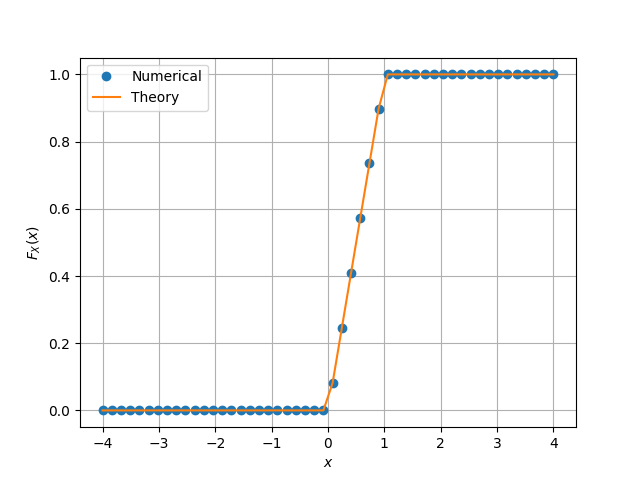
\includegraphics[width=\columnwidth]
    {uni_cdf.png}
    \caption{}
    \label{fig1}
\end{figure}

\begin{lstlisting}
wget https://github.com/Deepshikha11004/Random_variable.git/codes/cdf_plot.py
\end{lstlisting}


\item
Find a  theoretical expression for $F_{U}(x)$.


\textbf{Solution:}
\begin{align}
   f_u(x)=
  \begin{cases}
  1 & 0<x<1\\
  0 & \text otherwise
  \end{cases}
\end{align}
For $x\le 0$,
\begin{align}
      F_u(x)&=\int_{-\infty}^{0} 0 dx \\
        &=0
\end{align}

For $0<x<1$,
\begin{align}
      F_u(x)&=\int_{0}^{x} 1 dx \\
        &=x
\end{align}

For $x \ge 1$,
\begin{align}
      F_u(x)&=\int_{1}^{\infty} 0 dx \\
        &=0
\end{align}

\item
The mean of $U$ is defined as
%
\begin{equation}
E\sbrak{U} = \frac{1}{N}\sum_{i=1}^{N}U_i
\end{equation}
%
and its variance as
%
\begin{equation}
\text{var}\sbrak{U} = E\sbrak{U- E\sbrak{U}}^2 
\end{equation}

Write a C program to  find the mean and variance of $U$. 


\textbf{Solution:}
\begin{lstlisting}
wget https://github.com/Deepshikha11004/Random_variable/blob/main/codes/main.c
wget https://github.com/Deepshikha11004/Random_variable/blob/main/codes/coeffs.h
\end{lstlisting}



\item Verify your result theoretically given that
\end{enumerate}

\begin{equation}
E\sbrak{U^k} = \int_{-\infty}^{\infty}x^kdF_{U}(x)
\end{equation}


\textbf{Solution:}

\begin{align}
    E[U^k] &=  0 + \int_{0}^{1} x^k dF_U(x) + 0 \\
                 &= \frac{1}{k + 1}  \\
    \implies E[U] &= \frac{1}{2}\\
                        &= 0.50\\
             E[U^2] &= \frac{1}{3}
\end{align}
Hence,
\begin{align}
    \text{Variance} &= E[U^2] - {{E[U]}}^2 \\
                    &= \frac{1}{3} - \brak{\frac{1}{2}}^2 \\
                    &= \frac{1}{12} \\
                    &= 0.0833
\end{align}

For $x \ge 1$,
\begin{align}
    E[U^k]&=\int_{0}^{\infty} x^k dF_u(x)\\
    &=0
\end{align}

\section{Central Limit Theorem}
%
\begin{enumerate}[label=\thesection.\arabic*
,ref=\thesection.\theenumi]

%
\item
Generate $10^6$ samples of the random variable
%
\begin{equation}
X = \sum_{i=1}^{12}U_i -6
\end{equation}
%
using a C program, where $U_i, i = 1,2,\dots, 12$ are  a set of independent uniform random variables between 0 and 1
and save in a file called gau.dat.

\textbf{Solution:}
\begin{lstlisting}
wget https://github.com/Deepshikha11004/Random_variable/blob/main/codes/main.c
wget https://github.com/Deepshikha11004/Random_variable/blob/main/codes/coeffs.h
\end{lstlisting}

%
\item
Load gau.dat in python and plot the empirical CDF of $X$ using the samples in gau.dat. What properties does a CDF have?


\textbf{Solution:}
The CDF of a random variable U has the following properties:

\begin{enumerate}
    \item $F_U(x)$ is a non-decreasing function of x where $-\infty<x<\infty$
    \item $F_U(x)$ ranges from 0 to 1
    \item $F_U(x)$ = 0 as x$\rightarrow$ -$\infty$
    \item $F_U(x)$ = 1 as x$\rightarrow$ $\infty$
\end{enumerate}
The CDF of $X$ is plotted in Fig.2using the code below
\begin{lstlisting}
wget https://github.com/Deepshikha11004/Random_variable/blob/main/codes/x_cdf_plot.py
\end{lstlisting}
\begin{figure}[!ht]
    \centering
    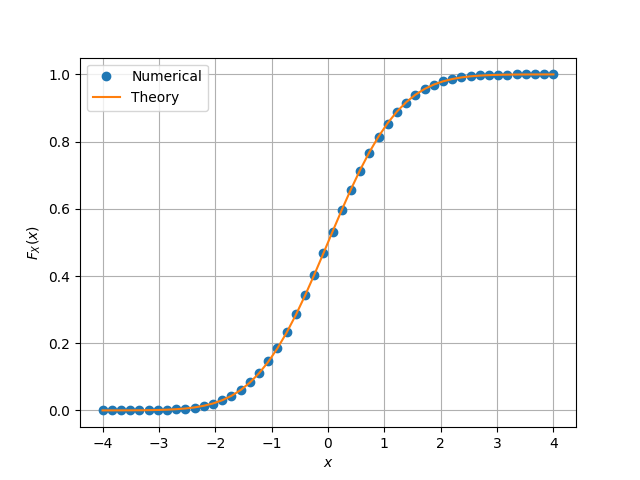
\includegraphics[width=\columnwidth]
    {x_cdf.png}
    \caption{}
    \label{fig2.2}
\end{figure}

\item
Load gau.dat in python and plot the empirical PDF of $X$ using the samples in gau.dat. The PDF of $X$ is defined as
\begin{align}
p_{X}(x) = \frac{d}{dx}F_{X}(x)
\end{align}
What properties does the PDF have?


\textbf{Solution:}
The PDF of a random variable X has the following properties:
\begin{enumerate}
    \item The probability density function is non-negative for all the possible values. 
    \item $ \int_{-\infty}^{\infty} f\brak{x} \,dx  = 1 $ 
    \item $f\brak{x} = 0$ as $x \rightarrow -\infty$
    \item $f\brak{x} = 0$ as $x \rightarrow \infty$
\end{enumerate}
The PDF of $X$ is plotted in Fig.3 using the code below
\begin{lstlisting}
wget  https://github.com/Deepshikha11004/Random_variable/blob/main/codes/pdf_plot.py
\end{lstlisting}
\begin{figure}[!ht]
    \centering
    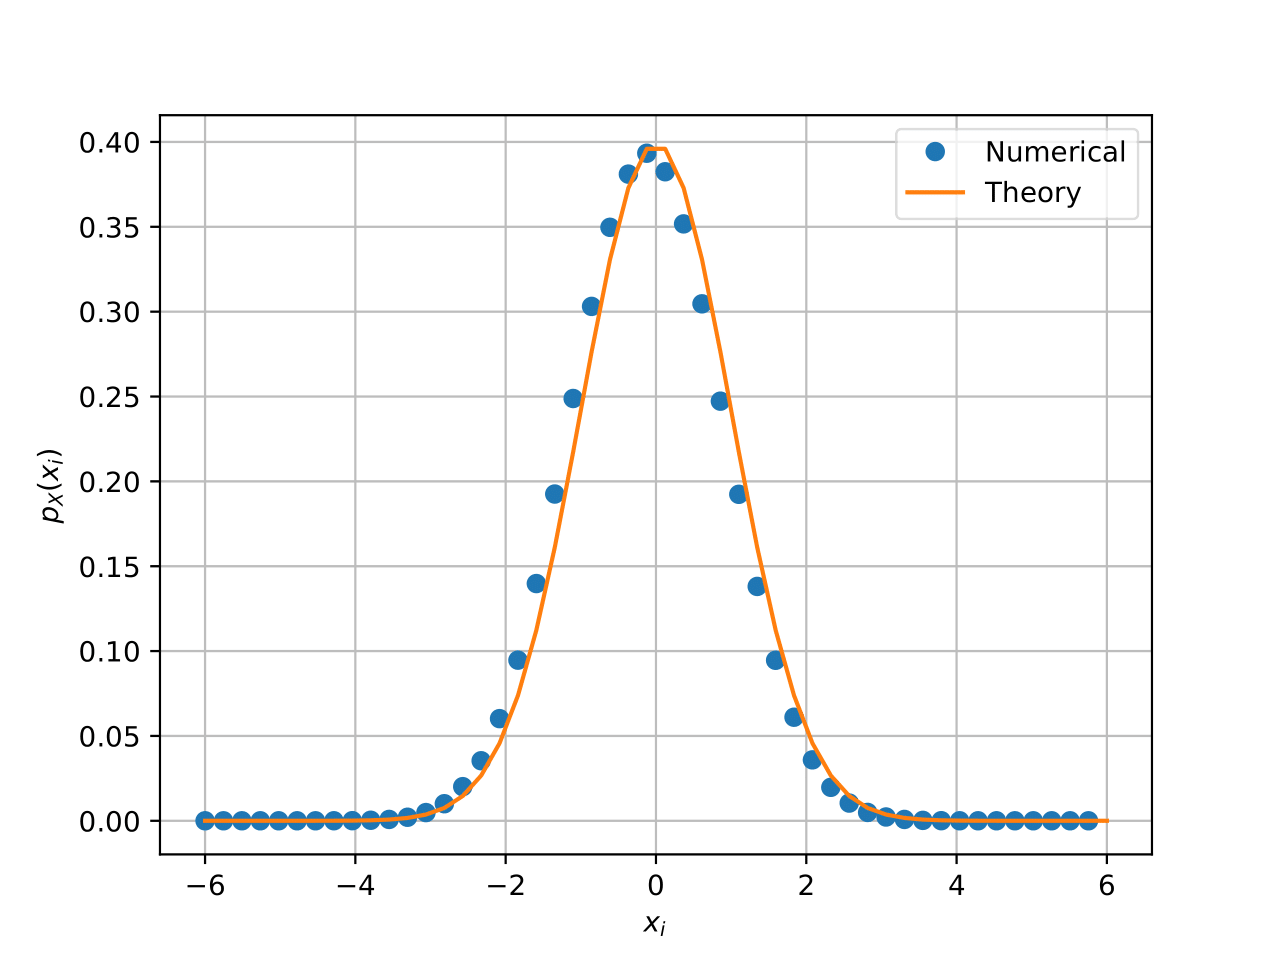
\includegraphics[width=\columnwidth]
    {gauss_pdf-1.png}
    \caption{}
    \label{fig3}
\end{figure}


\item Find the mean and variance of $X$ by writing a C program.


\textbf{Solution:}
\begin{lstlisting}
wget https://github.com/Deepshikha11004/Random_variable.git/codes/main.c
wget https://github.com/Deepshikha11004/Random_variable.git/codes/coeffs.h
\end{lstlisting}

\item Given that 
\begin{align}
p_{X}(x) = \frac{1}{\sqrt{2\pi}}\exp\brak{-\frac{x^2}{2}}, -\infty < x < \infty,
\end{align}
repeat the above exercise theoretically.


\textbf{Solution:}
\begin{align}
    F_X(x)&=\int_{-\infty}^{\infty} p_X(x) dx\\
    &=\int_{-\infty}^{\infty} \frac{1}{\sqrt{2\pi}}exp(\frac{-x^2}{2}) dx\\
    &=\frac{1}{\sqrt{2\pi}} \sqrt{2\pi}\Big|_{-\infty}^{\infty}\\
    &=1
\end{align}
By definition,
\begin{equation}
    p_X(x) dx=dF_U(x)
\end{equation}
Hence,
\begin{align}
    E[X]&=\int_{-\infty}^{\infty} x p_X(x) dx\\
       &=\int_{-\infty}^{\infty} x \frac{1}{\sqrt{2\pi}}exp(\frac{-x^2}{2}) dx\\
       &=0
\end{align}
Also,
\begin{equation}
\text{Variance}=E[X^2]-{{E[X]}^2}
\end{equation}
\begin{align}
    E[X^2]&=\int_{-\infty}^{\infty} x^2 p_X(x) dx\\
          &=\int_{-\infty}^{\infty} x^2 \frac{1}{\sqrt{2\pi}}exp(\frac{-x^2}{2}) dx\\
          &=\int_{-\infty}^{\infty} x x\frac{1}{\sqrt{2\pi}}exp(\frac{-x^2}{2}) dx\\
          &=\frac{1}{\sqrt{2\pi}}(-x exp(\frac{-x^2}{2})\Big|_{-\infty}^{\infty} +\int_{-\infty}^{\infty} exp(\frac{-x^2}{2})dx)\\
          &=\frac{1}{\sqrt{2\pi}}(0 +\sqrt{2\pi})\\
          &=1
\implies\text{Variance}=1
\end{align}
%
\end{enumerate}
\section{From Uniform to Other}
\begin{enumerate}[label=\thesection.\arabic*
,ref=\thesection.\theenumi]
%
\item
Generate samples of 
%
\begin{equation}
V = -2\ln\brak{1-U}
\end{equation}
%
and plot its CDF.  

\textbf{Solution:}
The following code generates samples of V in vdis.dat:
\begin{lstlisting}
wget https://github.com/Deepshikha11004/Random_variable/blob/main/codes/main.c
wget https://github.com/Deepshikha11004/Random_variable/blob/main/codes/coeffs.h
\end{lstlisting}
The following code plots CDF of V:
\begin{lstlisting}
wget https://github.com/Deepshikha11004/Random_variable/blob/main/codes/v_cdf_plot.py
\end{lstlisting}
\begin{figure}[!ht]
    \centering
    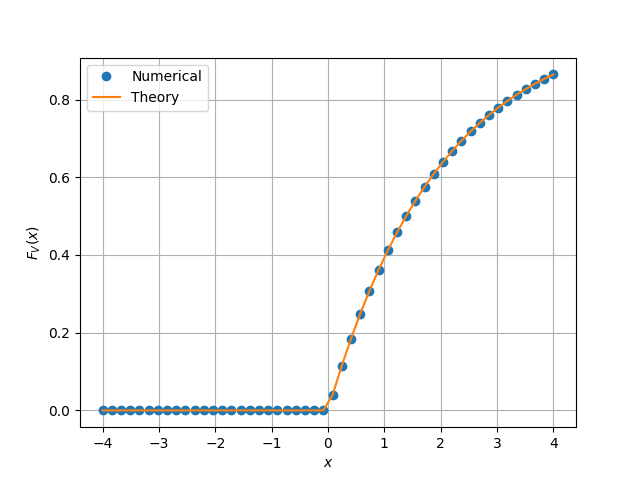
\includegraphics[width=\columnwidth]
    {v_cdf.png}
    \caption{}
    \label{fig1}
\end{figure}


\item Find a theoretical expression for $F_V(x)$.


\textbf{Solution:}
Let, $V = g\brak{U}$
\begin{align}
    V &= -2\ln{(1 - U)} \\
    \implies U &= 1 - e^{-\frac{V}{2}}
\end{align}
Now, 
\begin{align}
    F_{V}\brak{x} &= P\brak{g\brak{U}\leq x} \\
                  &= P\brak{X < g^{-1}\brak{V}} \\
                  &= F_{U}\brak{g^{-1}\brak{V}} \\
                  &= F_{U}\brak{1 - e^{-\frac{V}{2}}}
\end{align}
\begin{align}  
F_{U}\brak{1 - e^{-\frac{V}{2}}} = 
\begin{cases}
1 - e^{-\frac{V}{2}}, & V \in (0,\infty) \\
0, & \text{otherwise}
\end{cases}
\end{align}
\end{enumerate}

\section{Triangular Distribution}
\begin{enumerate}[label=\thesection.\arabic*
,ref=\thesection.\theenumi]
%
\item Generate 
	\begin{align}
		T = U_1+U_2
	\end{align}

\textbf{Solution:}	
Download  and run the code to generate tri.dat file.
\begin{lstlisting}
wget https://github.com/Deepshikha11004/Random_variable/blob/main/codes/main.c
wget https://github.com/Deepshikha11004/Random_variable/blob/main/codes/coeffs.h
\end{lstlisting}

	
\item Find the CDF of $T$.


\textbf{Solution:}
The CDF of T is plotted in Fig4 using the code given below:
\begin{lstlisting}
wget https://github.com/Deepshikha11004/Random_variable/blob/main/codes/t_cdf_plot2.py
\end{lstlisting}
\begin{figure}[!ht]
    \centering
    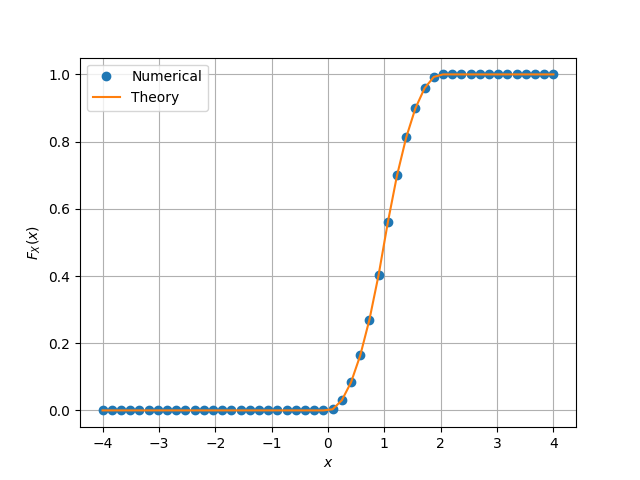
\includegraphics[width=\columnwidth]
    {t_cdf2.png}
    \caption{}
    \label{fig3}
\end{figure}





\item Find the PDF of $T$.


\textbf{Solution:}
\begin{figure}[!ht]
    \centering
    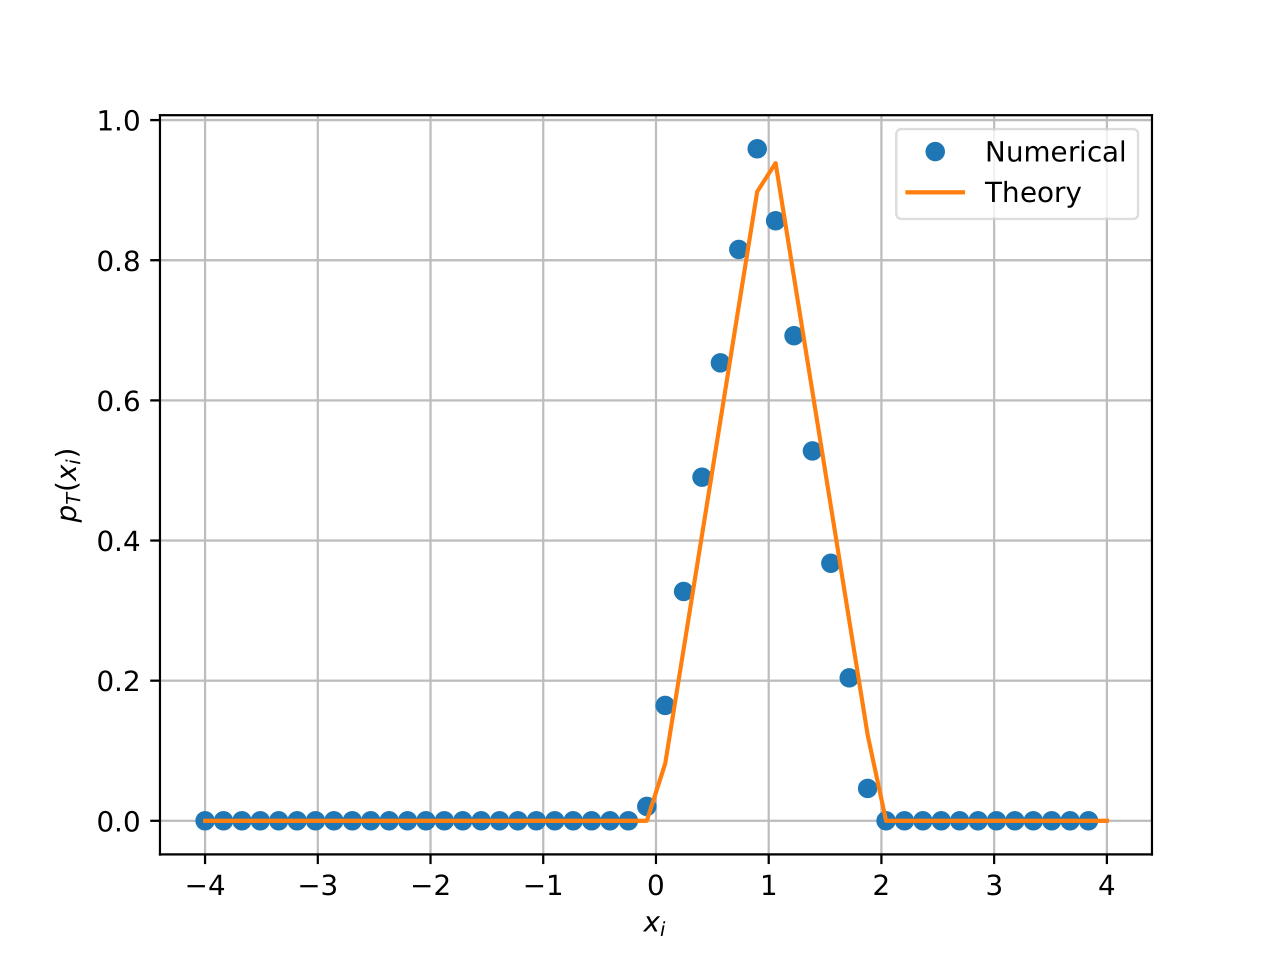
\includegraphics[width=\columnwidth]
    {tri_pdf-1.png}
    \caption{}
    \label{fig3}
\end{figure}



\textbf{Solution:}
The PDF of T is plotted in Fig4 using the code given below:
\begin{lstlisting}
wget https://github.com/Deepshikha11004/Random_variable/blob/main/codes/t_pdf_plot.py
\end{lstlisting}


\item Find the theoretical expressions for the PDF and CDF of $T$.


\textbf{Solution:}
\begin{align}
    p_T(T) &= p_{U_1 + U_2}(T) = p_{U_1}(T) * p_{U_2}(T)\\
     T&=U_1 +U_2\\
 \implies   p_T(x) &= \int_{-\infty}^{\infty}p_{U_1}(U_2)p_{U_2}(T-U_1) d U_1\\
    p_T(T) &= \int_0^1p_{U_1}(T-U_1) d U_1
\end{align}
For $T<0$,
\begin{align}
    p_T(T)=0
\end{align}
For $0 \ge T < 1$,
\begin{align}
    p_T(T)&=\int_{0}^{T} d U_2\\
    &=T
\end{align}
For $1 \ge T < 2$,
\begin{align}
    p_T(T)&=\int_{T-1}^{2} d U_2\\
    &=2-T
\end{align}
For $T>2$,
\begin{align}
    p_T(T)=0
\end{align}
Therefore,

\begin{align}
    \displaystyle p_T(T) = \begin{cases} 
    0 & \text otherwise\\  
    T & \text{$0 < x < 1$} \\  
    2 - T & \text{$1 \leq x < 2$} 
    \end{cases}
\end{align}
Now,
\begin{align}
    F_T(T)=\int p_T(T) dx
\end{align}
Therefore,
\begin{align}
    \displaystyle F_T(x) = \begin{cases} 
    0 & \text otherwise \\  
    \frac{T^2}{2} & \text{$0 < T < 1$} \\  
    -\frac{T^2}{2} + 2T - 1 & \text{$1 \leq T < 2$} 
    \end{cases}
\end{align}

\item Verify your results through a plot. 


\textbf{Solution:}
Done in 4.2 and 4.3.
\end{enumerate}
\section{Maximul Likelihood}
\begin{enumerate}[label=\thesection.\arabic*
,ref=\thesection.\theenumi]
\item Generate equiprobable $X \in \cbrak{1,-1}$.


\textbf{Solution:}
Run the main.c file to generate 'ber.dat' file.
\begin{lstlisting}
wget https://github.com/Deepshikha11004/Random variable/blob/main/codes/main.c
wget https://github.com/Deepshikha11004/Random variable/blob/main/codes/coeffs.h
\end{lstlisting}
\item Generate 
\begin{equation}
Y = AX+N,
\end{equation}
where $A = 5$ dB,  and $N \sim \mathbb{N}(0, 1)$.

\textbf{Solution:}
Run the main.c file to generate 'maxlike.dat' file.
\begin{lstlisting}
wget https://github.com/Deepshikha11004/Random variable/blob/main/codes/main.c
wget https://github.com/Deepshikha11004/Random variable/blob/main/codes/coeffs.h
\end{lstlisting}
	\item Plot $Y$ using a scatter plot.
	
	
\textbf{Solution:}
\begin{figure}[!ht]
    \centering
    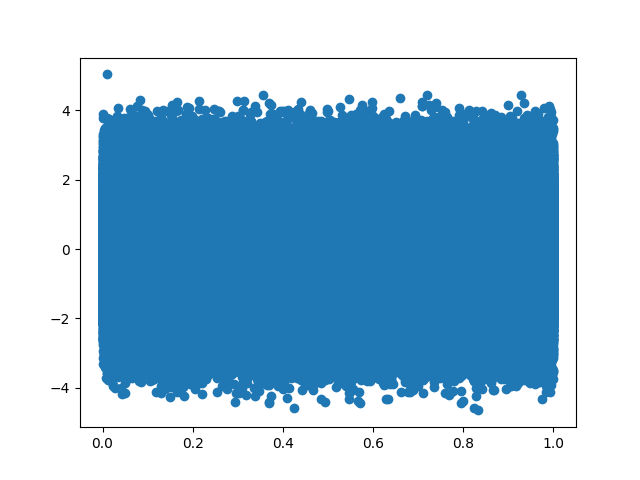
\includegraphics[width=\columnwidth]
    {Y_scatter.png}
    \caption{}
    \label{fig3}
\end{figure}
The Y scatter plot is generated using 'maxlike.dat' file using the following code:
\begin{lstlisting}
wget https://github.com/Deepshikha11004/Random variable/blob/main/codes/scatter_plot.py
\end{lstlisting}


\item Guess how to estimate $X$ from $Y$.


\textbf{Solution:}
We have,
\begin{align}
    Y=AX+N
\end{align}
Estimation of X from Y :
\begin{align}
    \hat{X}=sgn(Y)
\end{align}
where,
\begin{align}
    sgn(Y)=
    \begin{cases}
       -1 & ;-\infty<y<0\\
        1 & ; 0<y<\infty
    \end{cases} 
\end{align}

\item
\label{ml-ch4_sim}
Find 
\begin{equation}
	P_{e|0} = \pr{\hat{X} = -1|X=1}
\end{equation}
and 
\begin{equation}
	P_{e|1} = \pr{\hat{X} = 1|X=-1}
\end{equation}

\textbf{Solution:}
Run the following code and using the function'$x_cap$' we get the required values.
\begin{lstlisting}
    wget https://github.com/Deepshikha11004/Random variable/blob/main/codes/main.c
    wget https://github.com/Deepshikha11004/Random variable/blob/main/codes/coeffs.h

\end{lstlisting}
\begin{align}
    P_{e|0}&=0.310536\\
    P_{e|1}&=0.310530
\end{align}

%
\item Find $P_e$ assuming that $X$ has equiprobable symbols.


\textbf{Solution:} 
      \begin{align}
        P_e=&\frac{P_{e|0}+P_{e|1}}{2}\\
        &=\frac{0.310536+0.310530}{2}\\
        &=0.310533
      \end{align}
\item
Verify by plotting  the theoretical $P_e$ with respect to $A$ from 0 to 10 dB.  


\textbf{Solution:}
\begin{figure}[!ht]
    \centering
    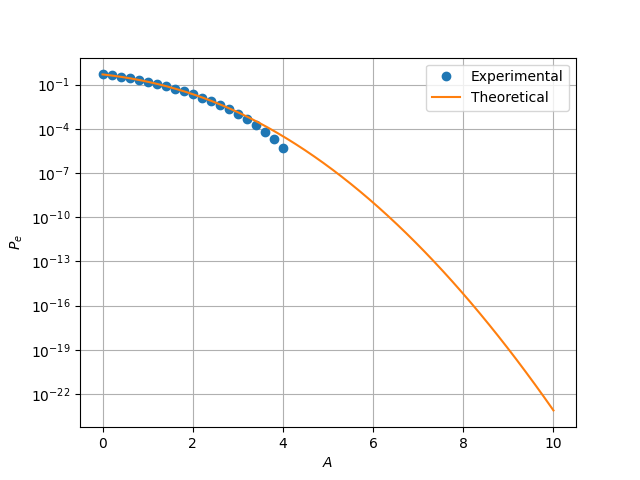
\includegraphics[width=\columnwidth]
    {p_e.png}
    \caption{}
    \label{fig5}
\end{figure}
\item Now, consider a threshold $\delta$  while estimating $X$ from $Y$. Find the value of $\delta$ that maximizes the theoretical $P_e$.


\textbf{Solution} We can define our guess as
        \begin{equation}
            \hat{X} = \begin{cases}
                1 & Y \geq \delta \\
                -1 & Y < \delta
            \end{cases}
        \end{equation}
        Now,
        \begin{align}
            P_{e|0} &= \pr{\hat{X} = -1 | X = 1} \\
            &= \pr{AX + N < \delta | X = 1} \\
            &= \pr{A + N < \delta} \\
            &= \pr{N < -A + \delta} \\
            &= F_N(-(A - \delta)) \\
            &= Q(A - \delta)
        \end{align}
        Similarly,
        \begin{equation}
            P_{e|1} = Q(A + \delta)
        \end{equation}
        So we have,
        \begin{align}
        \begin{split}
            P_e &= P_{e|0} \cdot \pr{X = -1} \\
            &\quad+ P_{e|1} \cdot \pr{X = 1}
        \end{split} \\
            &= Q(A - \delta) \cdot \frac{1}{2} + Q(A + \delta) \cdot \frac{1}{2} \label{eq:p_e}
        \end{align}
        To find the minimal $P_e$, we differentiate Eq \eqref{eq:p_e} wrt $\delta$ and equate it to
        0
        \begin{align}
            0 &= \frac{d}{d\delta}\left(\frac{1}{2}\left(Q(A-\delta) + Q(A+\delta)\right)\right) \\
            &= \frac{1}{2} \frac{1}{\sqrt{2\pi}}
                \left(e^{-\frac{(A-\delta)^2}{2}} - e^{-\frac{(A+\delta)^2}{2}}\right)
        \end{align}
        So we have
        \begin{align}
            (A - \delta)^2 &= (A + \delta)^2 \\
            \implies \delta &= 0
        \end{align}
        Therefore, $P_e$ is minimal when the threshold is ,$\delta = 0$.

\item Repeat the above exercise when 
	\begin{align}
		p_{X}(0) = p
	\end{align}


    \textbf{Solution:} We have
        \begin{align}
            P_e &= P_{e|0} p + P_{e|1} (1 - p) \\
            &= Q(A - \delta) p + Q(A + \delta) (1 - p)
        \end{align}
        Differentiating wrt $\delta$ to get minimum,
        \begin{align}
            0 &= \frac{d}{d\delta}(Q(A - \delta) p + Q(A + \delta) (1 - p)) \\
            &= pe^{-\frac{(A - \delta)^2}{2}} - (1 - p) e^{-\frac{(A + \delta)^2}{2}}
        \end{align}
        Taking $\ln$ on both sides,
        \begin{align}
            \ln{p} - \frac{(A - \delta)^2}{2} &= \ln(1 - p) - \frac{(A + \delta)^2}{2} \\
            2 A \delta &= \ln \frac{1 - p}{p} \\
            \delta &= \frac{1}{2 A} \ln \frac{1 - p}{p}
        \end{align}
       

    

    
\item Repeat the above exercise using the MAP criterion.

\textbf{Solution:}Assume $\pr{X = -1} = p$.

        According to the MAP criterion, when
        \begin{equation}
            p_{X|Y}(-1|y) > p_{X|Y}(1|y) \label{eq:5.10:MAP}
        \end{equation}
        We should guess -1, else we guess 1. Now,
        \begin{equation}
            p_{X|Y}(x|y) = \frac{p_{Y|X}(y|x)p_X(x)}{p_Y(y)} \label{eq:5.10:x|y}
        \end{equation}
    
        Now,
        \begin{equation}
            p_{Y|X}(y|-1) = p_{(-A+N)}(y)
        \end{equation}
        Since $A$ is a constant,
        \begin{align}
            p_{Y|X}(y|-1) &= p_{N}(y + A) \\
            &= \frac{1}{\sqrt{2 \pi}}e^{-\frac{(y + A)^2}{2}}
        \end{align}
        Substituting into \eqref{eq:5.10:x|y},
        \begin{align}
            p_{X|Y}(-1|y) &= \frac{p_{Y|X}(y|-1)p_X(-1)}{p_Y(y)} \\
            p_{X|Y}(-1|y) &= \frac{\frac{1}{\sqrt{2 \pi}} e^{-\frac{(y+A)^2}{2}} p}{p_Y(y)}
                \label{eq:5.10:-1|y}
        \end{align}
        Similarly,
        \begin{align}
            p_{X|Y}(1|y) &= \frac{\frac{1}{\sqrt{2 \pi}} e^{-\frac{(y-A)^2}{2}} (1-p)}{p_Y(y)}
                \label{eq:5.10:1|y}
        \end{align}
        Finally, substituting Eqs \eqref{eq:5.10:-1|y} and \eqref{eq:5.10:1|y} into Eq
        \eqref{eq:5.10:MAP}, we should guess that $X = -1$ when
        \begin{align}
            \frac{\frac{1}{\sqrt{2 \pi}} e^{-\frac{(y+A)^2}{2}} p}{p_Y(y)}
                &> \frac{\frac{1}{\sqrt{2 \pi}} e^{-\frac{(y-A)^2}{2}} (1-p)}{p_Y(y)} \\
            \frac{p}{1-p} &> e^{2 A y} \\
            y &< \frac{1}{2A} \ln \frac{p}{1-p}
        \end{align}
        So we have our guess,
        \begin{equation}
            \hat{X} = \begin{cases}
                -1 & y < \delta \\
                1 & \text{otherwise}
            \end{cases}
        \end{equation}
        where $\delta = \frac{1}{2A} \ln \frac{p}{1-p}$.

        Considering the special case when $p=\frac{1}{2}$,
        \begin{align}
            \delta &= \frac{1}{2 A} \ln 1 \\
            \delta &= 0
        \end{align}
        So our guess is,
        \begin{equation}
            \hat{X} = \begin{cases}
                -1 & y < 0 \\
                1 & y > 0
            \end{cases}
        \end{equation}
		\end{enumerate}
\section{Gaussian to Other}
\begin{enumerate}[label=\thesection.\arabic*
,ref=\thesection.\theenumi]
\item
% Let $X_1 \sim  \gauss{0}{1}$ and $X_2 \sim  \gauss{0}{1}$. Plot the CDF and PDF of
%
\begin{equation}
V = X_1^2 + X_2^2
\end{equation}


\textbf{Solution:}
Run the following code to generate 'chi.dat' file.
\begin{lstlisting}
wget https://github.com/Deepshikha11004/Random variable/blob/main/codes/main.c
wget https://github.com/Deepshikha11004/Random variable/blob/main/codes/coeffs.h
\end{lstlisting}
\item
If
%
\begin{equation}
F_{V}(x) = 
\begin{cases}
1 - e^{-\alpha x} & x \geq 0 \\
0 & x < 0,
\end{cases}
\end{equation}
%
find $\alpha$.


\textbf{Solution:}
Define the random variables as:
\begin{align}
X_1&=R\cos\theta\\
X_2&=R\sin\theta
\end{align}
The Jacobian matrix is defined as:
\begin{align}
    J &= \begin{bmatrix}
        \frac{\partial X_1}{\partial R} & \frac{\partial X_1}{\partial \Theta} \\
        \frac{\partial X_2}{\partial R} & \frac{\partial X_2}{\partial \Theta}
    \end{bmatrix} \\
    J &= \begin{bmatrix}
        \cos \Theta & -R \sin \Theta \\
        \sin \Theta & R \cos \Theta
    \end{bmatrix} \\
    \implies |J| &= R 
\end{align}
Since,$X_1$ and $X_2$ are iid,
\begin{align}
    p_{X_1 X_2}(x_1,x_2)&=p_{X_1}x_1 p_{X_2}x_2\\
    &=\frac{1}{2\pi}exp(\frac{-(x_1^2 +x_2^2)}{2})\\
    &=\frac{1}{2\pi}exp(\frac{-r^2}{2})
\end{align}
We know that,
\begin{align}
    p_{R\theta}{(r,\theta)}=|J|p_{X_1 X_2}(x_1,x_2)
\end{align}
Therefore,
\begin{align}
    p_{R\theta}{(r,\theta)}&=\frac{r}{2\pi}exp(\frac{-r^2}{2})\\
    \implies p_{R}(r) &= \int_{0}^{2 \pi} p_{R, \Theta}(r, \theta) d \theta \\
            &= r e^{-{\frac{r^2}{2}}}
\end{align}
We have,
\begin{align}
    F_R(r) &= \int_{0}^{r} p_R(r) \\
    &= \int_{0}^{r} r e^{-\frac{r^2}{2}} dr \\
    &= \left(-e^{-\frac{r^2}{2}}\right)_{0}^{r} \\
    &= 1 - e^{-\frac{r^2}{2}}
\end{align}
and,
\begin{align}
    F_V(x) &= \pr{V \leq x} \\
    &= \pr{X_1^2 + X_2^2 \leq x} \\
    &= \pr{R^2 \leq x}
    &= \pr{R \leq \sqrt{x}} \\
    &= F_R(\sqrt{x}) \\
    &= 1 - e^{-\frac{x}{2}} \\
    &= 1 - e^{- \alpha x}
\end{align}
Hence we get,
        \begin{equation}
            \alpha = \frac{1}{2}
        \end{equation}



%
\item
\label{ch3_raleigh_sim}
Plot the CDF and PDf of
%
\begin{equation}
A = \sqrt{V}
\end{equation}

\textbf{Solution:}
Following is the code:
\begin{lstlisting}
wget https://github.com/Deepshikha11004/Random variable/blob/main/codes/chiroot_pdf.py
wget https://github.com/Deepshikha11004/Random variable/blob/main/codes/chiroot_cdf.py
\end{lstlisting}
These are the PDF and CDf plots:
\begin{figure}[!ht]
    \centering
    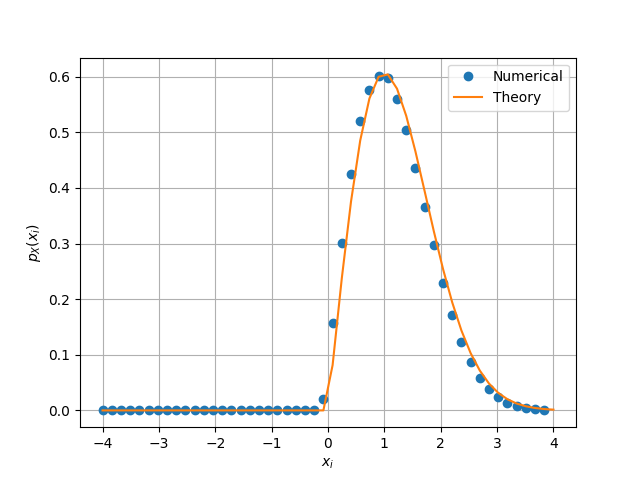
\includegraphics[width=\columnwidth]
    {root_V.png}
    \caption{}
    \label{fig6}
\end{figure}
\begin{figure}[!ht]
    \centering
    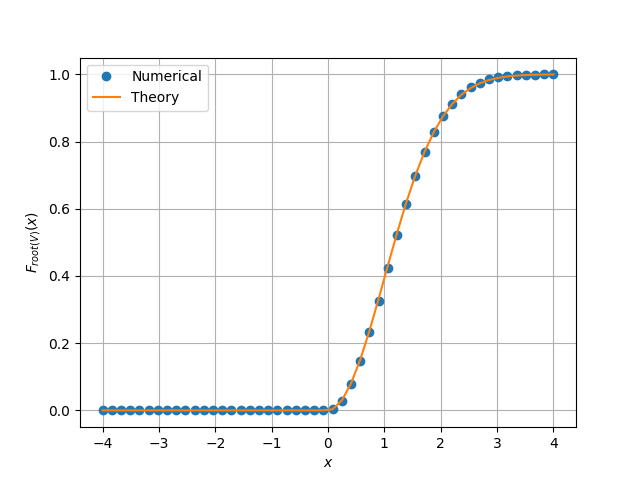
\includegraphics[width=\columnwidth]
    {rootV_cdf.png}
    \caption{}
    \label{fig6}
\end{figure}

\end{enumerate}

\section{Conditional Probability}
\begin{enumerate}[label=\thesection.\arabic*
,ref=\thesection.\theenumi]
\item
\item
\label{ch4_sim}
Plot 
\begin{equation}
P_e = \pr{\hat{X} = -1|X=1}
\end{equation}
%
for 
\begin{equation}
Y = AX+N,
\end{equation}
% where $A$ is Raleigh with $E\sbrak{A^2} = \gamma, N \sim \gauss{0}{1}, X \in \brak{-1,1}$ for $0 \le \gamma \le 10$ dB.

%
\item
Assuming that $N$ is a constant, find an expression for $P_e$.  Call this $P_e(N)$

%
\item
%
\label{ch4_anal}
For a function $g$,
\begin{equation}
E\sbrak{g(X)} = \int_{-\infty}^{\infty}g(x)p_{X}(x)\, dx
\end{equation}
%
Find $P_e = E\sbrak{P_e(N)}$.

%
\item
Plot $P_e$ in problems \ref{ch4_sim} and \ref{ch4_anal} on the same graph w.r.t $\gamma$.  Comment.

		\end{enumerate}
\section{Two Dimensions}
Let 
\begin{equation}
\mbf{y} = A\mbf{x} + \mbf{n},
\end{equation}
where 
\begin{align}
x &\in \brak{\mbf{s}_0,\mbf{s}_1}, 
\mbf{s}_0 = 
\begin{pmatrix}
1 
\\
0
\end{pmatrix},
\mbf{s}_1 = 
\begin{pmatrix}
0 
\\
1
\end{pmatrix}
\\
\mbf{n} &= 
\begin{pmatrix}
n_1
\\
n_2
\end{pmatrix},
% n_1,n_2 \sim \gauss{0}{1}.
\end{align}
%
\begin{enumerate}[label=\thesection.\arabic*
,ref=\thesection.\theenumi]

%%
\item
\label{ch5_fsk}
Plot 
%
\begin{equation}
\mbf{y}|\mbf{s}_0 \text{ and } \mbf{y}|\mbf{s}_1
\end{equation}
%
on the same graph using a scatter plot.

%
\item
For the above problem, find a decision rule for detecting the symbols $\mbf{s}_0 $ and $\mbf{s}_1$.

%
\item
Plot 
\begin{equation} 
P_e = \pr{\hat{\mbf{x}} = \mbf{s}_1|\mbf{x} = \mbf{s}_0}
\end{equation}
with respect to the SNR from 0 to 10 dB.

%
\item
Obtain an expression for $P_e$. Verify this by comparing the theory and simulation plots on the same graph.

%
		\end{enumerate}


\end{document}
